%-------------------------------------------------------------------------------
\section{Motivation}\label{s:motivation}
%-------------------------------------------------------------------------------

This section reviews the potential benefits of serverless for
interactive workloads such as web applications, and presents
evidence that the {\problem} will need to be solved in order to
obtain those benefits.

\subsection{Web applications are a good fit for serverless}

Serverless is well suited to situations where load can vary rapidly
and is hard to predict, so that long-term cloud resource reservations
would lead to waste during low-load periods. Web applications often
fit this profile.

For example, consider a web site with 50,000 requests per day, each
request consuming 200 ms of CPU time and 128 MB of memory. The web
site is bursty in the sense that it has work only about a fifth of the
time. Running this web site on AWS Lambda would cost about \$1.60 per
month. The cheapest EC2 instance (which reserves compute resources)
costs just over \$3 per month. The expense-minimizing choice differs
depending on load level and degree of
burstyness~\cite{econ-of-serverless,trek10-blog},
but generally high load variation favors serverless.

Slowly-changing load can be handled by dynamic adjustment to long-term
reserved resources (e.g. EC2 instances), but such adjustments can take
multiple minutes~\cite{ec2-autoscaling} and are thus not suited to
rapid load variation.

\subsection{The \problem{}}

\begin{figure}[t!]
    \centering
      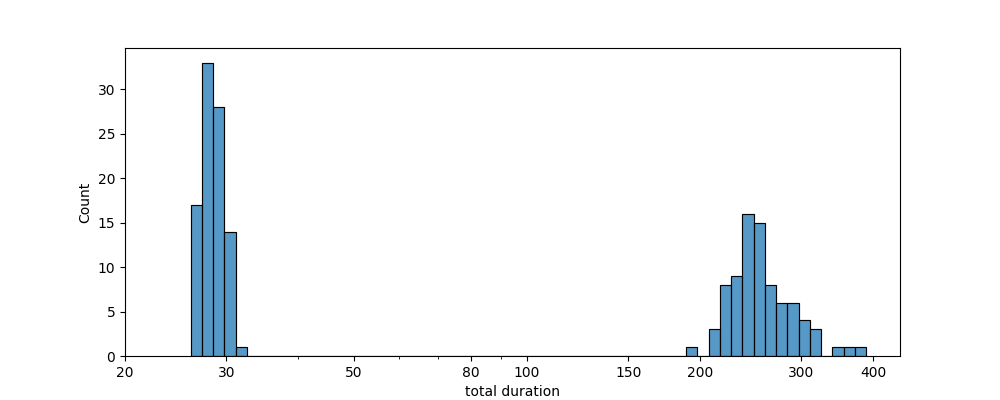
\includegraphics[width=8.5cm]{img/lambda_total_durations.png}
      \caption{Distribution of end-to-end durations for a simple function on AWS Lambda. The y axis is log scale. }
    \label{fig:lambda-total-durations}
\end{figure}

\begin{figure}[t!]
    \centering
      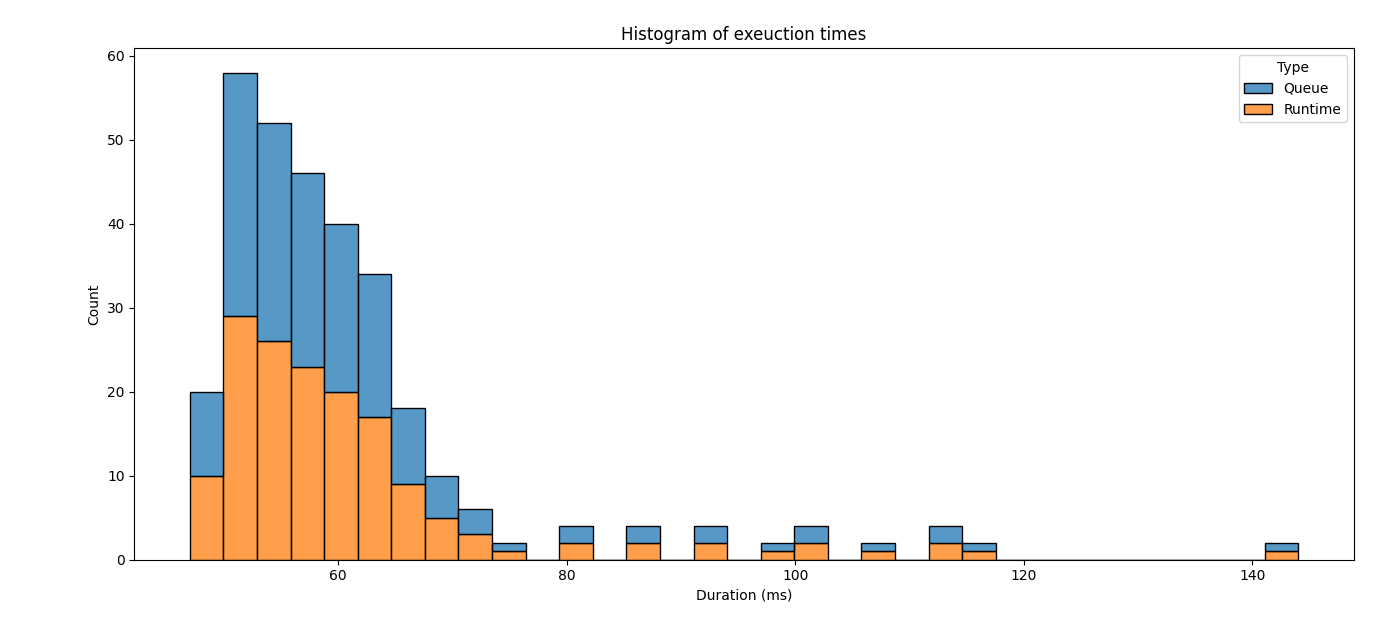
\includegraphics[width=8.5cm]{img/knative_stacked.png}
      \caption{Distribution of end-to-end durations broken down by
        queuing (blue) and runtime (orange) delay for a simple function on
        knative.}
    \label{fig:knative}
\end{figure}

Cloud providers are motivated to keep their compute hardware as busy
as possible, in order to avoid waste and reduce costs. In a
non-reservation system like serverless, if the average load is near
capacity (to minimize average waste), the peak load will be above
capacity, imposing either queuing or time-sharing delays on functions.

% an important part of the story is that we expect there to be
% lots of BE traffic, so that there is something to pre-empt 
% during bursts of LC work.

Measurements of cold-start delays in AWS Lambda show evidence
of
this \problem{}.
The experiment launches a test function at intervals randomly
spaced between 0 and 10 minutes; the function
just sleeps for 20ms and then returns. AWS Xray~\cite{aws-xray}
records end-to-end latencies.
The results are in Figure~\ref{fig:lambda-total-durations}. The spike
on the left side of the graph reflects warm-start executions,
which use a cached container left over from a previous execution.
We verify this by having each function look for some state changed
in the container by the previous invocation.

The right-hand grouping in Figure~\ref{fig:lambda-total-durations}
reflects invocations that required cold start (creation of a new
container). The delays have a wide spread, between $\sim$200 and
$\sim$400ms, suggesting that there is more going on than just creation
of a new container. One potential cause we can rule out is fetching
the container image from S3; such fetches have been measured to take
on the order of a second~\cite{sigmaos}; and this experiment uses a
generic Python container that is also used by many others on AWS
Lambda and thus likely cached. Though AWS Lambda is difficult to
investigate in detail, we can examine the designs of other serverless
systems to see whether the {\problem} would cause the kind of delay
variation in the graph.

Knative is popular open-source serverless system~\cite{knative}, which
runs a Kubernetes pod for each function; pods time-share the
provider's server. Knative assigns functions to pods until the pod is
fully loaded, and then queues the function until a pod has capacity or
the autoscaler has created new pod.  We run an experiment with Knative
in which we generate a steady stream of background functions and
periodically invoke a latency-sensitive function that computes for
50ms. Figure~\ref{fig:knative} shows the spread of end-to-end
durations for the latency-sensitive function.  The graph breaks down
the total duration into queuing and runtime (i.e., the time from the
first to last line of code of the function).  The graph shows that the
duration of latency-sensitive functions is affected by both
time-sharing and queuing: the \problem{}.

%% Knative~\cite{knative} similarly queues excess invocations, although it does
%% so via the load balancer, which is also in charge of
%% autoscaling~\cite{knative-sched}: if the existing pods are fully loaded (with a
%% small, bounded-size queue in front of them), requests are queued separately
%% while the autoscaler starts up more pods.

%% The OpenWhisk~\cite{openwhisk} load balancer chooses a machine to run
%% each new function on and adds a message to a Kafka queue addressed to
%% that machine; the machine pulls invocation messages as resources are
%% freed up by the termination of previous
%% functions~\cite{openwhisk-sched}. This means that 
%% a latency sensitive function might sit in the Kafka queue while
%% another tenant's background function completes: the \problem{}.

%% Hermod~\cite{hermod} is a recent research serverless scheduler, and shows in a
%% simulation that late binding (as Knative does) performs worse than
%% early binding. Under high load, Hermod places the excess functions on machines
%% anyway (used a least loaded policy) and does Processor Sharing scheduling among
%% them. This means that all are equally slowed down, and no one function has a
%% high delay. This still leads to the \problem{}: now rather than experiencing
%% queuing, latency sensitive functions experience time-sharing delay. Hermod does not
%% address what happens when the machines are out of memory. 

% I (rtm) don't understand this next paragraph, after the first sentence.

% None of these schedulers 
% know which functions to prioritize under high load.

% The way all of the above schedulers avoid the \problem{} is by doing different
% forms of accounting concurrency: concurrency can be reserved or provisioned
% for specific functions, and limited for others. This is necessary to ensure
% that a burst in background tasks doesn't starve the latency sensitive
% functions. Reserving and provisioning and limiting are, however, conceptually
% in tension with the goal of serverless, which is to be on-demand and flexible.



% It is impossible to know what proprietary systems like AWS do, but since AWS
% guarantees an amount of memory as well as a fraction of vCPUs to each function,
% it is likely AWS also queues the invocations to ensure they aren't put in a
% position of having to break those guarantees.\hmng{that might be a test we could
% run: do a tight while loop and look at cpu time and wall clock time to see how
% we are being scheduled} 
